\section{Performance test}
This section contains the results from the performance test done by the subjects. First of the results from the regressor trained only with EMG data are presented, and afterwards compared to the regressor trained with inclusion of IMU data. 

\begin{figure}[H]
	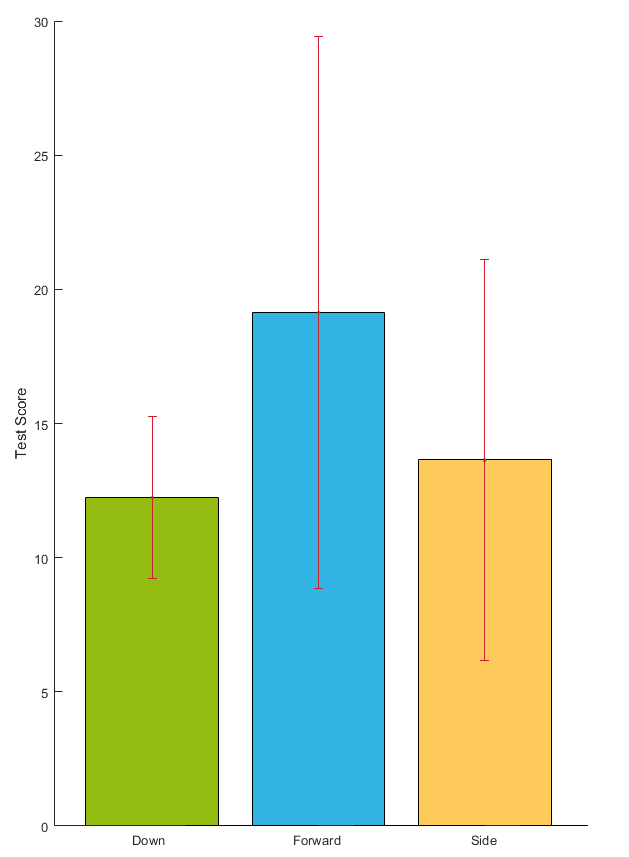
\includegraphics[width=0.5\textwidth]{figures/results/TestScore.png}  %<--but is not needed.
	\caption{Calculated performance scores of the regressors trained with the logarithmic variance feature for the three limb positions. The bar chart illustrates the mean score across all subjects, and the error bar illustrates the standard deviation.}
	\label{fig:TestScore}
\end{figure}

The mean performance score of the test in the downright limb position across all subjects is 12.2417 with a standard deviation of $\pm 3.0080$. For the forward limb position the mean score is 19.1381 with a standard deviation of $\pm 10.2966$, and for the side limb position the mean score is 13.6479 with a standard deviation of $\pm 7.4756$. 
